\documentclass[10pt,twocolumn,a4paper]{article}
\usepackage[margin=1.8cm,columnsep=0.7cm]{geometry}
\usepackage[T1]{fontenc}
\usepackage{mathptmx}
\usepackage{microtype}
\usepackage{amsmath,amssymb}
\usepackage{graphicx}
\usepackage{booktabs}
\usepackage{enumitem}
\usepackage{listings}
\usepackage{xcolor}
\usepackage{tikz}
\usetikzlibrary{arrows.meta,positioning}
\usepackage[font=small,labelfont=bf]{caption}
\usepackage{cite}
\usepackage[colorlinks=true,linkcolor=blue!50!black,citecolor=blue!50!black,urlcolor=blue!50!black]{hyperref}
\setlist{nosep,leftmargin=*}
\urlstyle{same}
\setlength{\parskip}{0pt}
\renewcommand{\arraystretch}{1.1}
\emergencystretch=2em

% MATLAB listing style (used in Appendix A, one-column page, so that no code line is wrapped)
\lstdefinestyle{mat}{language=Matlab,basicstyle=\ttfamily\fontsize{7.8}{9.3}\selectfont,
  keywordstyle=\color{blue!60!black}\bfseries,commentstyle=\color{green!35!black}\itshape,
  stringstyle=\color{violet},numbers=left,numberstyle=\tiny\color{gray},numbersep=6pt,
  breaklines=true,breakatwhitespace=false,columns=fullflexible,keepspaces=true,
  postbreak=\mbox{\textcolor{gray}{$\hookrightarrow$}\space},breakindent=8pt,
  frame=single,rulecolor=\color{gray!60},xleftmargin=16pt,framexleftmargin=14pt,
  showstringspaces=false,aboveskip=6pt,belowskip=4pt}

\title{\vspace{-0.8cm}\textbf{Industrial Machine Vibration Analysis\\Using Digital Signal Processing}}
\author{
PULI PRAGNAN , Dr. BHASKER DAPPURI\\[2pt]
160124735307, ECE -- III Year\\[2pt]
Department of Electronics and Communication Engineering\\[2pt]
Chaitanya Bharathi Institute of Technology (CBIT)
}
\date{}
\usepackage{titlesec}
% Section headings: 1. Introduction, 2. Problem Statement, etc.
\titleformat{\section}
  {\normalfont\large\bfseries}
  {\thesection.}
  {0.3em}
  {}
% Control vertical spacing around section headings
\titlespacing*{\section}{0pt}{4pt}{1pt}
\begin{document}
\twocolumn[
\maketitle
\vspace{-0.6cm}
\noindent
\begin{minipage}{\textwidth}
\noindent{\large\bfseries Abstract}\par
\vspace{2pt}
\noindent
A change in a machine's vibration spectrum can be an early sign of a developing fault. This undergraduate project presents a MATLAB implementation that demonstrates how basic digital signal processing (DSP) makes such a change visible. The script generates, in MATLAB, a synthetic ``healthy'' signal (30 and 60~Hz components) and a synthetic ``faulty'' signal (the same components plus illustrative 180 and 300~Hz components), adds white Gaussian noise, smooths both signals with a 5-point moving-average (MA) filter, computes single-sided FFT amplitude spectra, and compares the two cases through their spectra, their RMS values, and their spectral energy in a 150--220~Hz band. \textbf{All signals are MATLAB-generated synthetic signals; no real industrial machine was recorded or tested.} The script contains no threshold, classifier or automatic decision rule, and it is not a real-time system. The script was executed in MATLAB R2025b and the three resulting figures were observed. In that run, the 150--220~Hz energy of the filtered faulty signal was 0.1894, compared with 0.0278 for the filtered healthy signal (about 6.8 times), while the RMS values were 0.8356 and 0.7836 (a difference of about 6.6\%). The MA filter also attenuates the fault components; its theoretical gains are 0.708 at 180~Hz and 0.312 at 300~Hz. The methods are standard textbook techniques, and no new algorithm is claimed.

\vspace{3pt}
\noindent\textbf{Keywords:} vibration monitoring, condition monitoring, synthetic signals, moving-average filter, FFT, spectral band energy, MATLAB
\end{minipage}
\vspace{0.2cm}
]

\section{Introduction}
Rotating machines such as motors, pumps and fans are central to industry. When a fault develops (unbalance,
misalignment, looseness, wear), the machine's vibration usually changes, often before the machine fails, so measuring
vibration is a standard way to monitor machine condition~\cite{randall}. Standards such as ISO~20816-1 give general
guidelines for measuring and evaluating machine vibration~\cite{iso}.

A raw vibration waveform is difficult to judge by eye because it mixes noise with several frequencies. DSP helps in
two ways: a filter can reduce part of the noise, and the Fourier transform shows which frequencies are present and
how strong they are~\cite{oppenheim,proakis}. This project applies these two tools in the simplest way so that every
step can be run, understood and explained. It is a teaching demonstration on synthetic data, not a validated
monitoring system.

\section{Problem Statement}
A noisy vibration waveform is hard to interpret directly. The problem addressed here is to show, on controlled synthetic
signals, how a simple filter and the FFT make a change in frequency content visible, and how a small number of
numerical features (RMS value and band energy) respond to that change.

\section{Objectives}
\begin{enumerate}
\item Generate a synthetic healthy signal and a synthetic faulty signal that contains additional fault-related frequency components.
\item Add random noise and reduce part of it with a moving-average filter.
\item Plot the signals before and after filtering, and compute their single-sided FFT spectra.
\item Compare the healthy and faulty filtered spectra, and compute two simple features: the RMS value and the spectral energy in a 150--220~Hz band.
\item State clearly what the script does not do (Section~\ref{sec:limits}).
\end{enumerate}

\section{Proposed Solution and System Block Diagram}
Fig.~\ref{fig:block} shows the processing chain implemented in the script. The same chain is applied to the healthy and
the faulty signal, so any difference between their outputs comes from the signals and not from the processing.

\begin{figure}[t]
\centering
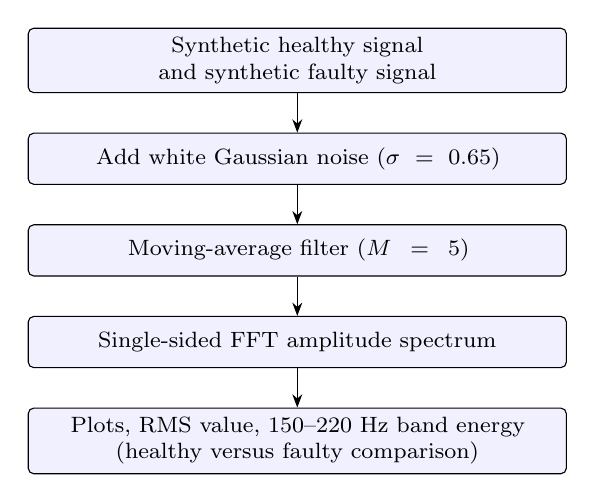
\begin{tikzpicture}[node distance=5mm,
 b/.style={draw,rounded corners=2pt,align=center,font=\footnotesize,minimum height=6.5mm,text width=6.6cm,fill=blue!6}]
\node[b](a){Synthetic healthy signal and synthetic faulty signal};
\node[b,below=of a](b){Add white Gaussian noise ($\sigma=0.65$)};
\node[b,below=of b](c){Moving-average filter ($M=5$)};
\node[b,below=of c](d){Single-sided FFT amplitude spectrum};
\node[b,below=of d](e){Plots, RMS value, 150--220~Hz band energy\\(healthy versus faulty comparison)};
\foreach \i/\j in {a/b,b/c,c/d,d/e}{\draw[-{Stealth}] (\i) -- (\j);}
\end{tikzpicture}
\caption{Block diagram of the processing chain in the MATLAB script.}\label{fig:block}
\end{figure}

\textbf{From input to output.}
\begin{enumerate}
\item \emph{Signals.} A healthy signal and a faulty signal are generated synthetically (Section~\ref{sec:signals}).
\item \emph{Noise.} Independent white Gaussian noise is added to each signal.
\item \emph{Filtering.} Each noisy signal is smoothed with a 5-point moving average.
\item \emph{Spectrum.} The single-sided FFT amplitude spectrum is computed for each signal before and after filtering.
\item \emph{Comparison.} The filtered healthy and faulty spectra are plotted together, and the RMS value and the energy in the 150--220~Hz band are printed for both filtered signals.
\end{enumerate}
The output is three figures and four printed numbers (two features for each of the two signals). The script makes no NORMAL/FAULT decision.

\section{DSP Methodology}
\subsection{Synthetic signals}\label{sec:signals}
The sampling frequency is $f_s=2000$~Hz and the duration is $T=2$~s, giving $N=4000$ samples. The healthy signal is the sum of a
30~Hz component and a 60~Hz harmonic (amplitudes 1 and 0.30). The faulty signal adds two illustrative fault-related components at 180 and
300~Hz (amplitudes 0.55 and 0.30). These frequencies and amplitudes are chosen for illustration; they are not taken from a real
machine. All components have zero phase and fixed amplitude (Eq.~\ref{eq:sig}).

\subsection{Why a moving-average filter?}
Measurement noise changes quickly from sample to sample, while the machine components change smoothly. Averaging $M$ neighbouring
samples keeps the slow part and reduces much of the fast random part. It is one of the simplest low-pass filters and has a single parameter
($M=5$ here). Its cost is that it also weakens higher frequencies (Table~\ref{tab:gain}); a fault component at a high frequency is
reduced along with the noise.

\subsection{Why the FFT?}
In the waveform (Fig.~\ref{fig:time}) the components and the noise are added together. The FFT separates them by frequency, so the
strength at each frequency can be read directly, and a fault that creates new frequency content shows up as new spectral energy
(Figs.~\ref{fig:fft} and~\ref{fig:cmp}).

\subsection{A property of any linear filter}\label{sec:linear}
A linear filter multiplies the signal and the noise at the same frequency by the same gain $|H(f)|$, so it cannot improve the
signal-to-noise ratio at that frequency. It helps only by reducing noise at frequencies where there is little or no signal.
In the 150--220~Hz band used here, the mean of $|H(f)|^{2}$ is 0.481 (the factor applied to the noise energy), while the
180~Hz fault component is scaled by $|H(180)|^{2}=0.501$. These factors are comparable, so the filter should not
be expected to increase the contrast between healthy and faulty band energy (Section~\ref{sec:results}).

\section{Mathematical Equations}
\textbf{Synthetic signals.} For $n=0,\dots,N-1$,
\begin{align}
x_h[n] &= \sin\!\Big(2\pi\tfrac{30\,n}{f_s}\Big)+0.30\sin\!\Big(2\pi\tfrac{60\,n}{f_s}\Big),\nonumber\\
x_f[n] &= x_h[n]+0.55\sin\!\Big(2\pi\tfrac{180\,n}{f_s}\Big)+0.30\sin\!\Big(2\pi\tfrac{300\,n}{f_s}\Big).\label{eq:sig}
\end{align}
Here $f_s=2000$~Hz and $N=f_sT=4000$; amplitudes are in arbitrary units.

\textbf{Noise.} Let $x[n]$ denote either $x_h[n]$ or $x_f[n]$. Then
\begin{equation}
x_{\mathrm{noisy}}[n]=x[n]+v[n],\qquad v[n]\sim\mathcal N(0,\sigma^{2}).\label{eq:noise}
\end{equation}
$v[n]$ is artificial white Gaussian noise with $\sigma=0.65$ (MATLAB \texttt{randn}); the healthy and faulty signals receive independent noise
realizations.

\textbf{Moving-average filter.}
\begin{equation}
y[n]=\frac1M\sum_{m=-(M-1)/2}^{(M-1)/2}x_{\mathrm{noisy}}[n-m],\qquad M=5,\label{eq:ma}
\end{equation}
\begin{equation}
|H(f)|=\frac{\left|\sin(\pi f M/f_s)\right|}{M\left|\sin(\pi f/f_s)\right|}.\label{eq:H}
\end{equation}
The window length $M$ is odd, so the filter is centred and adds no delay. The code uses \texttt{conv(...,'same')}, which treats samples
outside the record as zero, so the first and last two output samples are affected by this edge effect. In Eq.~\eqref{eq:H}, $|H(f)|$ is the gain at frequency $f$;
it equals 1 at 0~Hz, decreases with $f$ up to $f_s/M=400$~Hz, where it is zero (it is also zero at the other multiples of $400$~Hz). For white noise, the output noise power is
$\sigma^{2}/M$, an improvement of $10\log_{10}M=6.99$~dB if the signal is not attenuated.

\textbf{Single-sided FFT amplitude spectrum.}
\begin{equation}
X[k]=\sum_{n=0}^{N-1}y[n]\,e^{-j2\pi kn/N},\qquad f_k=k\frac{f_s}{N},\label{eq:fft}
\end{equation}
\begin{equation}
A[k]=c_k\frac{|X[k]|}{N},\quad c_k=\begin{cases}1,&k=0,\ N/2,\\ 2,&k=1,\dots,N/2-1.\end{cases}\label{eq:amp}
\end{equation}
$A[k]$ is scaled so that a sine of amplitude $a$ shows height $a$. The bin spacing is $\Delta f=f_s/N=0.5$~Hz. All four signal
frequencies are multiples of 0.5~Hz and fall exactly on FFT bins, so no window is applied in this synthetic example.

\textbf{Features.}
\begin{equation}
E_{\mathrm{band}}=\sum_{k:\,150\le f_k\le 220}A[k]^{2},\qquad
\mathrm{RMS}=\sqrt{\frac1N\sum_{n=0}^{N-1}y[n]^{2}}.\label{eq:feat}
\end{equation}
The 150--220~Hz band contains 141 FFT bins and was chosen to contain the synthetic 180~Hz fault component; the 300~Hz component is
outside it. Both features are computed on the filtered signals.

\section{MATLAB Implementation}
\subsection{How to run}
\begin{enumerate}
\item Save the listing (or the supplied file) as \texttt{Industrial\_Machine\_Vibration\_DSP.m}.
\item In MATLAB press Run, or type the file name in the Command Window. The script uses only base MATLAB functions (\texttt{randn}, \texttt{conv},
\texttt{fft}, \texttt{subplot}, \texttt{plot}). The single-sided FFT function is a local function placed at the end of the script file;
MATLAB documents local functions in scripts from R2016b onward and, before R2024a, requires them to be at the end of the file, as they are here~\cite{mathworks}.
\item Three figure windows open and four numbers are printed in the Command Window. The script does not save figures or a log file.
\item The parameters (noise level, window length, band, duration) are set in the first lines of the script.
\end{enumerate}

\subsection{Execution status}\label{sec:verif}
The script in Appendix~\ref{app:code} was implemented and executed in MATLAB R2025b (version 25.2, Update~3), and the three figure windows it produces were observed.
The signals are generated by the script itself (Section~\ref{sec:signals}); they are synthetic, and no recording from a real industrial machine was used.
The four numbers in Table~\ref{tab:res} are the values printed in the MATLAB Command Window in that run, and Figs.~\ref{fig:time}--\ref{fig:cmp} are the figures
produced by the script in that run, exported from MATLAB without changes to their content. The script seeds the random generator with \texttt{rng(7)}, so the noise
is intended to be repeatable, but the exact noise-dependent values (RMS values and band energies) are those of the run reported here; a different seed would give somewhat different values.
The filter gains in Table~\ref{tab:gain} are computed analytically from Eq.~\eqref{eq:H} and do not depend on the random noise. They were not printed by the script.

\textbf{What was and was not tested.} Only this one execution of the script with the settings in the listing was carried out. No other seeds, noise levels, window lengths, signals or machines were tried, and no
real vibration data were processed.

\subsection{Complete code}
The complete script (114 lines) is given in Appendix~\ref{app:code} (Listing~\ref{lst:code}), after the references, exactly as executed; it is also delivered as a separate file.

\section{Results and Discussion}\label{sec:results}
\emph{All results are from synthetic signals generated by the MATLAB script, with artificial noise, and are taken from one execution in MATLAB R2025b (Section~\ref{sec:verif}). No real-machine data were used.}

\subsection{Signals before and after filtering}
Fig.~\ref{fig:time} shows the first 0.25~s of the healthy and faulty signals before and after the MA filter. Before filtering, both traces are dominated by rapid
sample-to-sample noise, with excursions of about $\pm3$ (read from the axes); the slow oscillation near 30~Hz (about seven to eight cycles in 0.25~s) is visible underneath it.
After smoothing, the traces are visibly smoother, the excursions are smaller (about $\pm2$), and the slow oscillation is much easier to see in both signals. The smoothed faulty trace appears
somewhat more irregular on each cycle than the smoothed healthy trace; this is a visual impression only and was not quantified. The vertical axis ranges differ between panels because MATLAB scaled each axis automatically.

\begin{figure*}[t]
\centering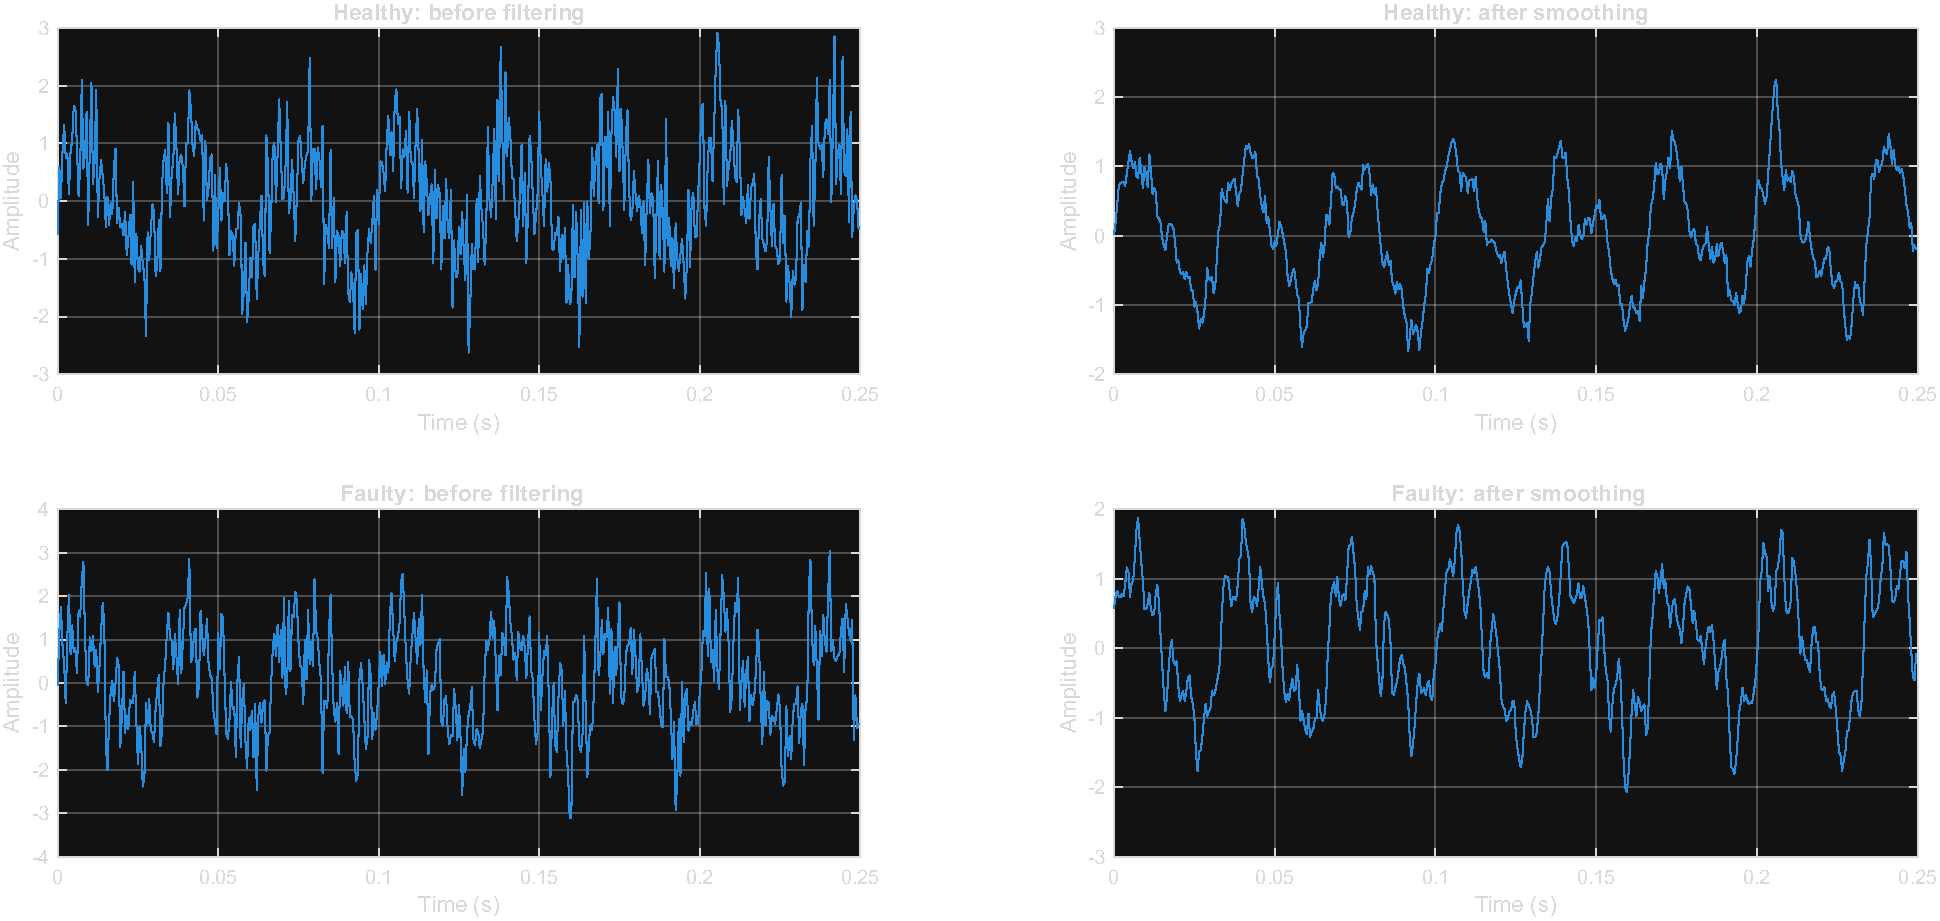
\includegraphics[width=0.95\textwidth]{fig_time.pdf}
\caption{Healthy (top) and faulty (bottom) synthetic vibration signals, before filtering (left) and after the 5-point MA filter (right), first 0.25~s. MATLAB R2025b output of the script in Appendix~\ref{app:code}.}\label{fig:time}
\end{figure*}

\begin{table}[t]
\centering\caption{Gain $|H(f)|$ of the $M=5$ moving-average filter at the four signal frequencies, computed analytically from Eq.~\eqref{eq:H} (independent of the random noise; not printed by the script).}\label{tab:gain}
\begin{tabular}{lcccc}\toprule
Frequency (Hz) & 30 & 60 & 180 & 300\\\midrule
Role & machine & machine & fault & fault\\
$|H(f)|$ & 0.991 & 0.965 & 0.708 & 0.312\\\bottomrule
\end{tabular}
\end{table}

\subsection{Spectra}
Fig.~\ref{fig:fft} shows the spectra before and after filtering. In the healthy case there are two clear peaks, at 30~Hz (magnitude close to 1) and at 60~Hz (about 0.3), on a low broadband noise floor.
In the faulty case the same two peaks are present, and two additional peaks appear at 180 and 300~Hz, which the healthy spectrum does not have. Before filtering, the faulty-case peaks at 180 and 300~Hz reach about 0.57 and 0.3;
after filtering they are lower, at about 0.4 and 0.09 (values read approximately from the plots). The 300~Hz peak is reduced proportionally much more than the 180~Hz peak, as expected from Table~\ref{tab:gain}. The broadband noise floor is
similar before and after filtering at low frequencies but is clearly lower after filtering at higher frequencies, where it falls close to zero near 400~Hz, consistent with the zero of $|H(f)|$ at $f_s/M=400$~Hz. Fig.~\ref{fig:cmp}
overlays the filtered healthy and filtered faulty spectra; they coincide at 30 and 60~Hz and on the noise floor, and differ at 180 and 300~Hz, where only the faulty spectrum shows peaks.

\begin{figure*}[t]
\centering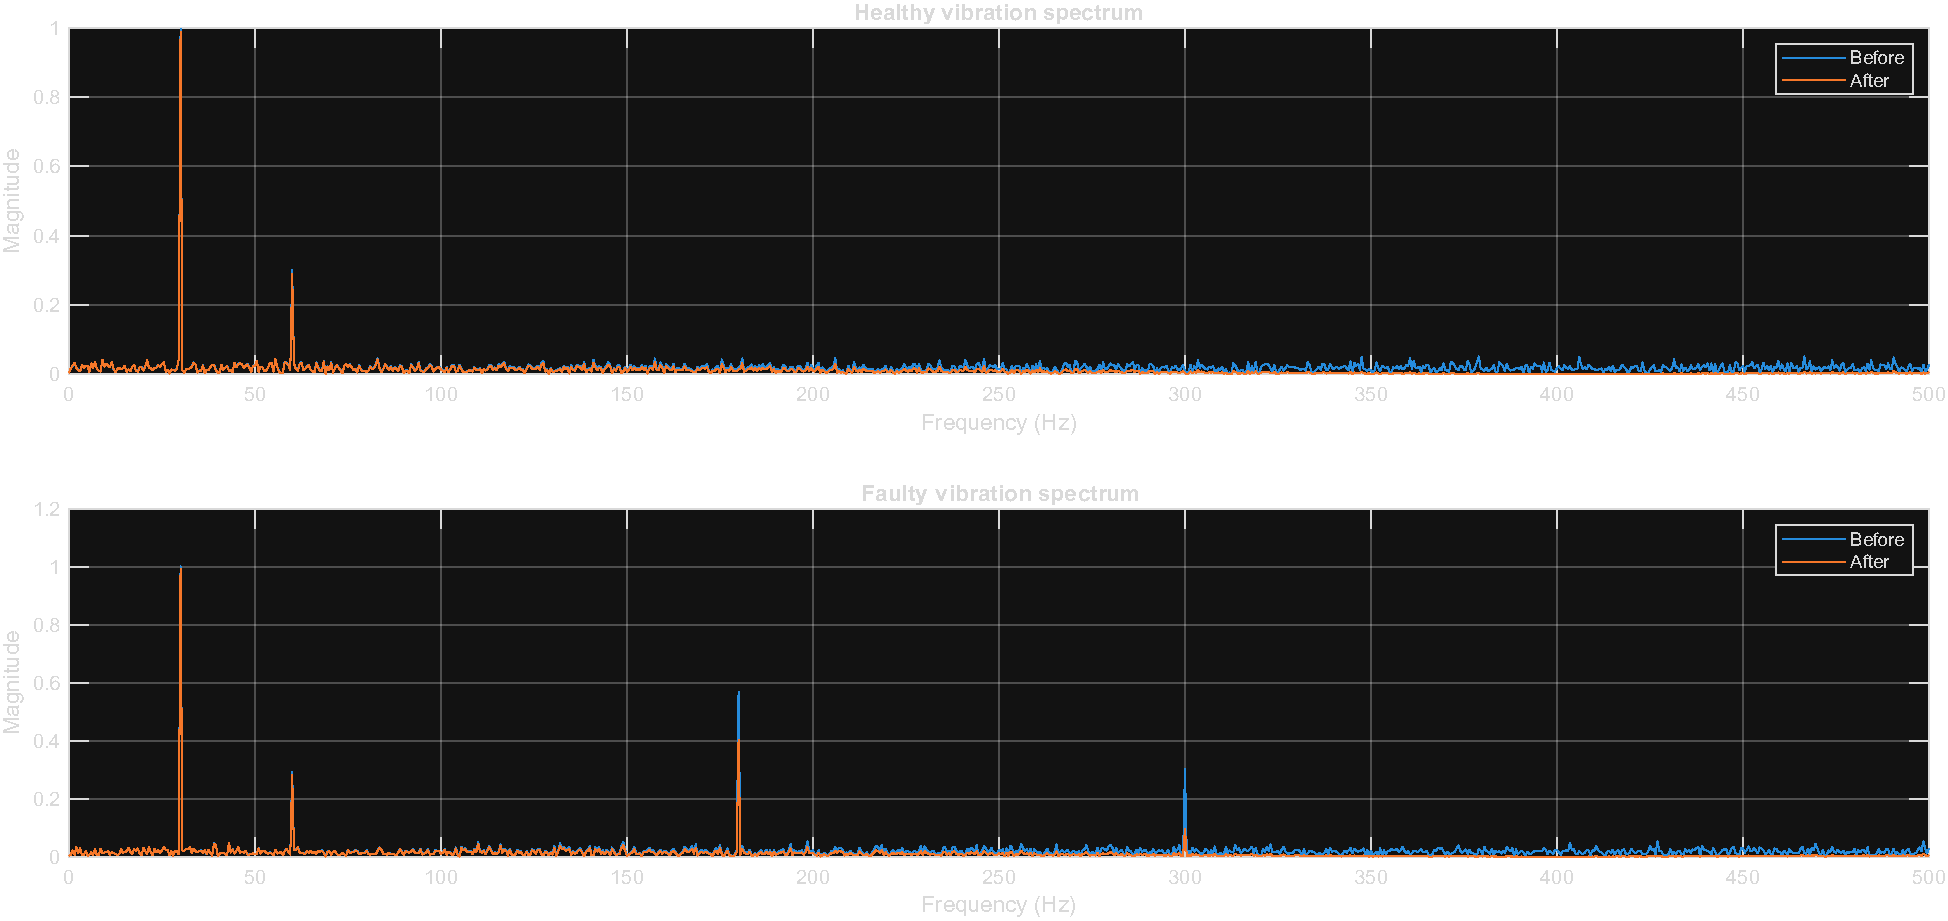
\includegraphics[width=0.95\textwidth]{fig_fft.pdf}
\caption{Single-sided FFT amplitude spectra (``Magnitude'') before and after MA filtering: healthy (top) and faulty (bottom), 0--500~Hz. MATLAB R2025b output of the script in Appendix~\ref{app:code}.}\label{fig:fft}
\end{figure*}

\begin{figure*}[t]
\centering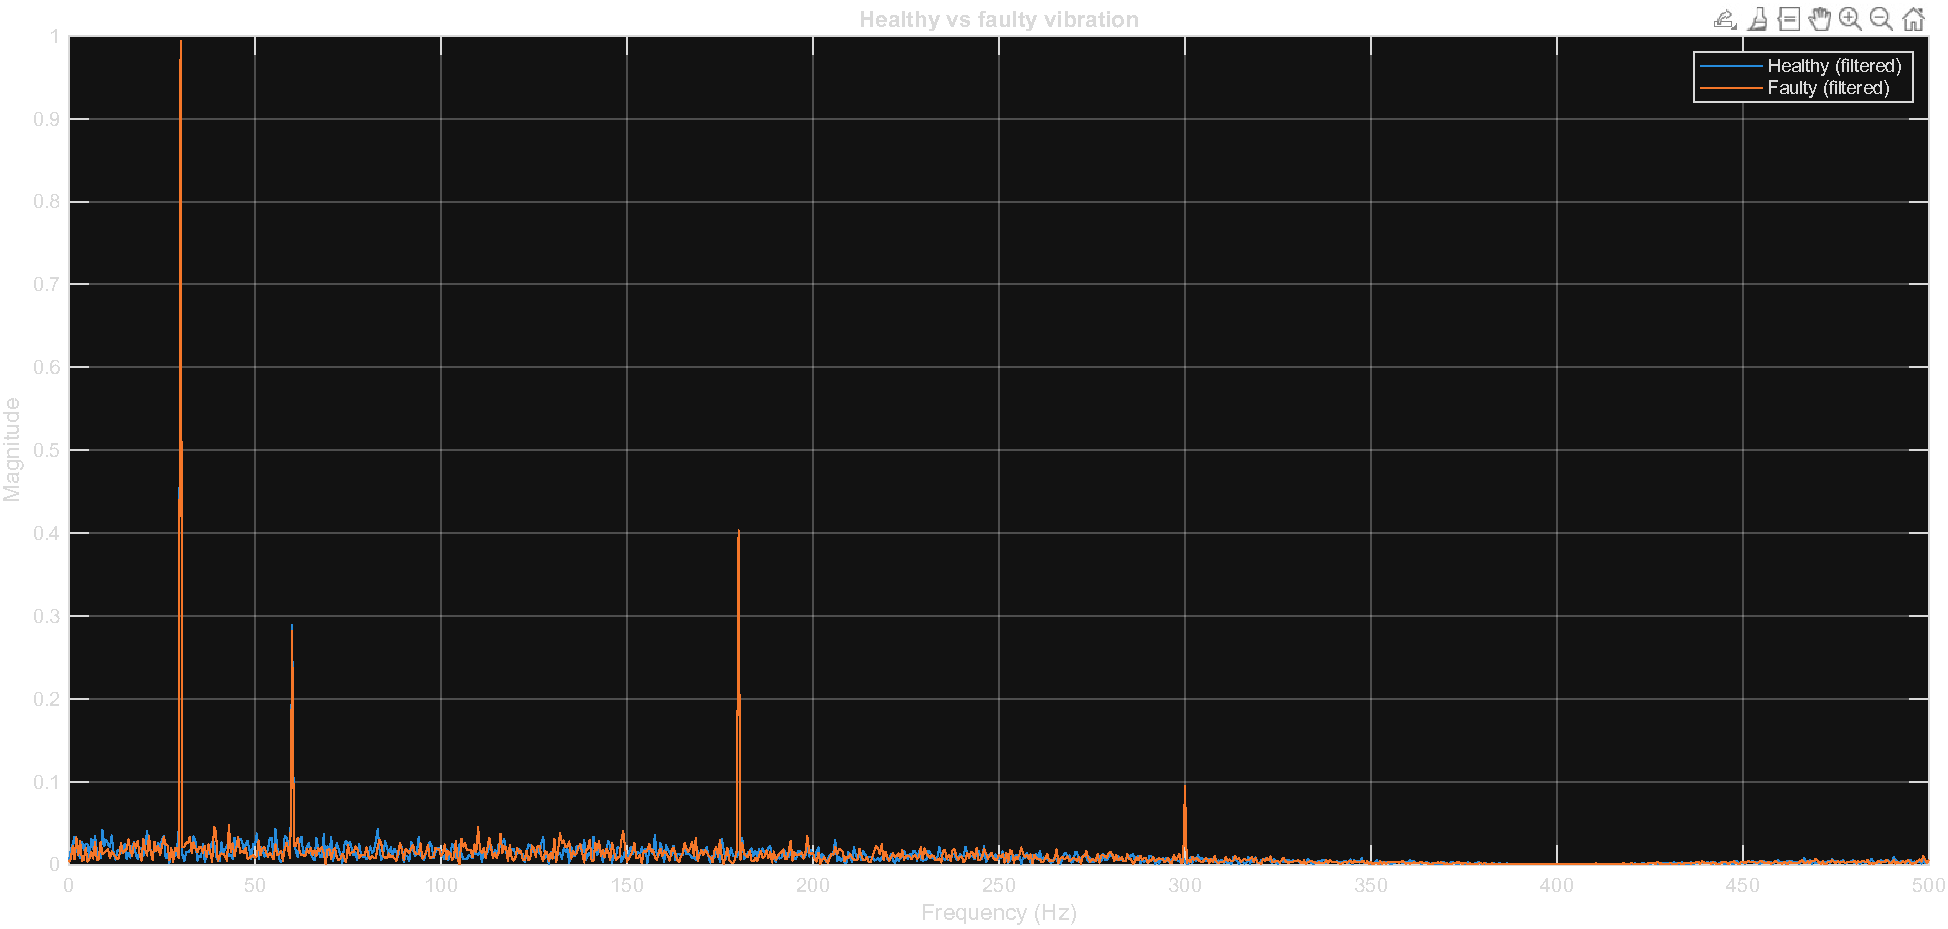
\includegraphics[width=0.95\textwidth]{fig_cmp.pdf}
\caption{Filtered healthy and filtered faulty spectra, 0--500~Hz. MATLAB R2025b output of the script in Appendix~\ref{app:code}.}\label{fig:cmp}
\end{figure*}

\subsection{Feature comparison}\label{sec:feat}
Table~\ref{tab:res} lists the four values printed by the script in MATLAB. The 150--220~Hz band energy of the faulty signal is about 6.8 times that of the healthy signal
($0.189427/0.027807\approx6.8$), whereas the RMS value is only about 6.6\% higher (0.8356 versus 0.7836). In this run the band energy is therefore a much more
sensitive indicator of this particular synthetic fault than the overall RMS value, because the fault adds energy at a few specific frequencies while the machine components at 30 and 60~Hz dominate the RMS.

\begin{table}[t]
\centering\caption{Values printed in the MATLAB R2025b Command Window by the script for the filtered signals (synthetic data; one noise realization, \texttt{rng(7)}).}\label{tab:res}
\begin{tabular}{lcc}\toprule
Quantity & Healthy & Faulty\\\midrule
Filtered RMS & 0.7836 & 0.8356\\
150--220~Hz spectral energy & 0.027807 & 0.189427\\\bottomrule
\end{tabular}
\end{table}

\textbf{Consistency check with theory.} The band energy can also be estimated analytically. For white noise of standard deviation $\sigma=0.65$, the expected energy over the $K=141$ bins before filtering is
$4\sigma^{2}K/N=0.0596$; the mean of $|H(f)|^{2}$ over the band is 0.481, so about 0.0287 is expected after filtering. Adding the filtered 180~Hz component, $(0.55\times0.708)^{2}=0.152$,
gives about 0.180 for the faulty signal. The MATLAB values, 0.0278 and 0.1894, are within about 3\% and 5\% of these estimates. Each printed value comes from a single noise realization and scatters around its expectation,
so exact agreement is not expected, and this single run does not by itself show how large that scatter is.

\subsection{Effect of the moving-average filter}
The filter reduces the broadband noise at higher frequencies (Fig.~\ref{fig:fft}) and the waveform becomes smoother (Fig.~\ref{fig:time}), but it also reduces
the fault components by the factors in Table~\ref{tab:gain}. Because the script does not compute the features without filtering, it provides no
numerical comparison of the band energy with and without the filter, so no claim is made here about whether filtering improves the separation between healthy and faulty
signals. The linear-filter property of Section~\ref{sec:linear} suggests that it need not.

\section{Applications, Limitations and Conclusion}
\subsection{Applications}
In its present form the script serves as a teaching demonstration of noise, filtering, the FFT and spectrum comparison.
Applying a similar chain to real recordings, with features chosen from a machine's own fault frequencies, is possible in
principle, but it would first require testing and validation on real machine data, which has not been done here.

\subsection{Limitations}\label{sec:limits}
\begin{itemize}
\item \textbf{Synthetic data only.} The signals, faults and noise are generated by the MATLAB script. No real machine was recorded or tested, and the approach is not validated on industrial machines.
\item \textbf{No decision rule and no real-time operation.} The script has no healthy reference set, threshold, classifier, or fault-detection rate. It does not output NORMAL or FAULT, and it does not identify fault type or location. It processes one stored two-second record per run and is not a real-time monitoring system.
\item \textbf{Single noise realization.} One healthy and one faulty signal are generated per run, with independent noise, so the printed numbers vary with the random seed. The script estimates no statistical spread, and only one execution was carried out.
\item \textbf{Frequency-specific feature.} The 150--220~Hz band was chosen because the synthetic fault contains a 180~Hz component. The 300~Hz component is not covered, and for real machines the band must be chosen from knowledge of the machine.
\item \textbf{Moving average attenuates high frequencies.} Fault signatures at several hundred Hz or higher would be weakened by the filter.
\item \textbf{No window function.} None is used. This is acceptable here because every component falls exactly on an FFT bin, but real recordings generally require a window before the FFT~\cite{harris}.
\item \textbf{Single execution.} The reported values and figures come from one execution of the script in MATLAB R2025b; no repeated trials, other seeds or parameter sweeps were performed.
\item \textbf{Not novel.} Moving averaging, the FFT and band-energy features are standard techniques.
\end{itemize}

\subsection{Conclusion}
A MATLAB script was implemented and executed (MATLAB R2025b) that generates synthetic healthy and faulty vibration signals, adds noise, smooths them with a
5-point moving-average filter, computes single-sided FFT spectra, and compares the two cases through their spectra, RMS values and
150--220~Hz band energy. In the observed run, the faulty signal showed extra spectral peaks at 180 and 300~Hz and a band energy of 0.1894 against 0.0278 for the healthy signal (about 6.8 times),
while the RMS value changed by only about 6.6\%. The filter reduced the noise at higher frequencies but also attenuated the fault components. These results concern synthetic, MATLAB-generated signals from a single execution only.
No real machine was recorded, and no real-time operation, real-machine testing or validated fault detection is claimed. Before any statement about practical performance can be made, the
approach must be tested on real machine recordings, with repeated trials and a justified decision rule.

\begin{thebibliography}{9}
\bibitem{randall} R. B. Randall, \emph{Vibration-based Condition Monitoring: Industrial, Aerospace and Automotive Applications}. Chichester, U.K.: Wiley, 2011, ISBN 978-0-470-74785-8.
\bibitem{iso} \emph{Mechanical vibration --- Measurement and evaluation of machine vibration --- Part 1: General guidelines}, ISO 20816-1:2016, International Organization for Standardization, Geneva, Switzerland, Nov. 2016.
\bibitem{oppenheim} A. V. Oppenheim and R. W. Schafer, \emph{Discrete-Time Signal Processing}, 3rd ed. Upper Saddle River, NJ, USA: Pearson, 2010.
\bibitem{proakis} J. G. Proakis and D. G. Manolakis, \emph{Digital Signal Processing: Principles, Algorithms, and Applications}, 4th ed. Upper Saddle River, NJ, USA: Pearson Prentice Hall, 2007.
\bibitem{mathworks} MathWorks, ``Add functions to scripts,'' MATLAB Documentation. [Online]. Available: \url{https://www.mathworks.com/help/matlab/matlab_prog/local-functions-in-scripts.html}. Accessed: Oct. 10, 2026.
\bibitem{harris} F. J. Harris, ``On the use of windows for harmonic analysis with the discrete Fourier transform,'' \emph{Proc. IEEE}, vol. 66, no. 1, pp. 51--83, Jan. 1978.
\end{thebibliography}

\onecolumn
\appendix
\section{Complete MATLAB Script}\label{app:code}
The listing below is the file \texttt{Industrial\_Machine\_Vibration\_DSP.m} exactly as executed in MATLAB R2025b; it has not been modified for this paper.

\lstinputlisting[style=mat,caption={\texttt{Industrial\_Machine\_Vibration\_DSP.m}: complete MATLAB script (114 lines).},label={lst:code}]{Industrial_Machine_Vibration_DSP.m}
\end{document}
